
\documentclass[CTN,lsstdraft,authoryear,toc]{lsstdoc}
\input{meta}

% Package imports go here.
\usepackage{amsmath}
\usepackage{hyperref}
\usepackage{graphicx}	% Including figure files
\usepackage{csquotes}

% Local commands go here.
\newcommand{\eq}[1]{\begin{equation}#1\end{equation}}
\newcommand{\ead}[1]{\begin{aligned}#1\end{aligned}}


%If you want glossaries
%\input{aglossary.tex}
%\makeglossaries

\title{Camera Shutter Motion Analysis}

% This can write metadata into the PDF.
% Update keywords and author information as necessary.
\hypersetup{
    pdftitle={Camera Shutter Motion Analysis},
    pdfauthor={Shuang Liang},
    pdfkeywords={}
}

% Optional subtitle
% \setDocSubtitle{A subtitle}

\input{authors}

\setDocRef{CTN-002}
\setDocUpstreamLocation{\url{https://github.com/lsst/ctn-002}}

\date{\vcsDate}

% Optional: name of the document's curator
% \setDocCurator{The Curator of this Document}

\setDocAbstract{%
Profile fitting for camera shutter trajectory and timing analysis.
}

% Change history defined here.
% Order: oldest first.
% Fields: VERSION, DATE, DESCRIPTION, OWNER NAME.
% See LPM-51 for version number policy.
\setDocChangeRecord{%
  \addtohist{1}{2025-07-16}{First Draft}{Shuang Liang}
}


\begin{document}

% Create the title page.
\maketitle
% Frequently for a technote we do not want a title page  uncomment this to remove the title page and changelog.
% use \mkshorttitle to remove the extra pages

\section{Data Structure}
The shutter motion profiles are located at
\begin{displayquote}
lsstcam-dc01.cp.lsst.org:/data/ccs-ipa-data/OBS\_DAY/SEQ\_NUM/
\end{displayquote}
and for each sequence number there're two motion profiles:
\begin{displayquote}
SEQ\_NUM\_shutterMotionProfileOpen.json, and  \\ SEQ\_NUM\_shutterMotionProfileClose.json.
\end{displayquote}
As the names suggest, each file corresponds to an open/close motion of one of the two shutter blades: PLUSX and MINUSX.
Some related meta information can be found in each file:
\begin{itemize}
    \item[] startTime: motion start time.
    \item[] startPosition: position of blade when motion started.
    \item[] targetPosition: target end positition.
    \item[] endPosition: action end position.
    \item[] targetDuration: target duration of motion.
    \item[] actionDuration: action duration of motion.
    \item[] side: ``PLUSX'' or ``MINUSX'', labeling two blades of the shutter.
\end{itemize}
In addition, two sets of measurement of the shutter motion (time and position) are included: encodeSamples and hallTransitions, as well as the fitted motion parameters: motorEncoderFit and hallSensorFit.  The following sections explain the fitting model in detail.

\section{Preparing for Fitting}
Both the motor encoder and the Hall sensors measure time stamps in TAI timescale and provided in both ISO and MJD format.  We first subtract the startTime to get a relative timing,
\begin{equation}
    t \to t - \mathrm{startTime},
\end{equation}
then append the end measurement (actionDuration, endPosition) as the last pair of the motion data ($t, s$). Next we normalize the time stamps by duration:
\eq{
    t \to t/\mathrm{actionDuration}.
}
Finally, the start position is subtracted from or subtracts the displacement $s$ depending on motion direction, and normalized by 750mm:
\eq{
	s \to
	\left\{ \ead{
			(s - \mathrm{startPosition})/750 \mathrm{mm} &, & \mathrm{endPosition} > \mathrm{startPosition}  \\
			(\mathrm{startPosition} - s)/750 \mathrm{mm} &, & \mathrm{endPosition} < \mathrm{startPosition}.  \\
}
\right.
}
In this set-up, the model always takes $t \approx [0,1]$ and maps to $s \approx [0,1]$, simplifying the fitting procedure. After the fitting, model parameters are scaled up to recover their physical units, with time parameters ($t_0, t_1, t_2$) multiplied by actionDuration, and jerk parameters ($j_0, j_1, j_2$) multiplied by $750 \cdot \mathrm{actionDuration}^{-3}$.

\section{Three Jerks Model v1}
The shutter motion profile is a piecewise constant jerk motion, as shown in Figure~\ref{fig:demo}.
\begin{figure*}
	\centering
        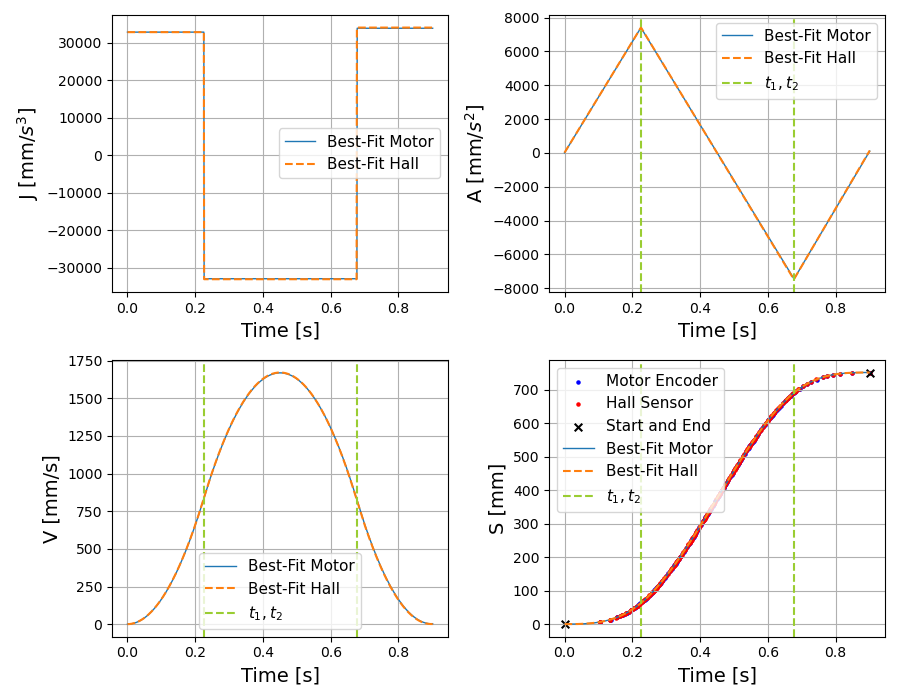
\includegraphics[width=0.99\hsize]{./figs/demo.png}
	\label{fig:demo}
    \caption{An example of a shutter motion profile. The plots show fitted jerk, acceleration, velocity and displacement respectively, of the  MINUSX-side blade open/PLUSX-side blade close. Motor encoder and Hall sensor measurements of the profile are also shown in the last panel.}
\end{figure*}
The position coordinate starts at $\sim0$mm from the PLUSX side and goes to $\sim750$mm at the MINUSX side. So when the MINUSX side opens/PLUSX side closes,  the shutter blade starts with a positive jerk $j_0$, then jumps to a negative jerk $j_1$ at a pivot time $t_1$, and jumps again to a positive jerk $j_2$ at the second pivot time $t_2$. For the other direction -- PLUSX side opens/MINUSX side closes -- the shutter experiences negative-positive-negative jerk jumps. But as the model is fitted on normalized data, it will always report positve-negative-positive jerks.

In addition to the above model parameters, a special parameter $t_0$ is introduced to measure a possible lag between the meta keyword startTime and the actual motion start time. The parameter essentially moves all measured time stamps by a tiny amount in order to better match a model profile that starts at 0. Notice that in the fitting, it is applied to the normalized time stamps,
\eq{
    t \to t - t_0,
}
but it is later scaled back to the unit of seconds and reported in the fitting results.

In summary, the three jerks model has 6 parameters:
\begin{itemize}
	\item[$t_0$:] Starting time of motion,
	\item[$t_1, t_2$:] Turning points for jerk and acceleration,
	\item[$j_0, j_1, j_2$:] The jerk for three intervals.
\end{itemize}
With patience, one can work out the math of the model:
\eq{
	j(t) =
	\left\{ \ead{
			j_0 &,& 0 < t < t_1 \\
			j_1 &,& t_1 < t < t_2 \\
			j_2 &,& t_2 < t < T,
}
\right.
}

\eq{
	a(t) =
	\left\{ \ead{
			j_0 t &,& 0 < t < t_1 \\
			a_1 + j_1 (t - t_1) &,& t_1 < t < t_2 \\
			a_2 + j_2 (t - t_2) &,& t_2 < t < T,
}
\right.
}
where $a_1 = a(t_1) = j_0 t_1$, and $a_2 = a(t_2) = a_1 + j_1 (t_2 - t_1) = j_0 t_1 + j_1 (t_2 - t_1).$ Re-organizing the terms,
\eq{
	a(t) =
	\left\{ \ead{
			j_0 t &,& 0 < t < t_1 \\
			A_1 + j_1 t &,& t_1 < t < t_2 \\
			A_2 + j_2 t &,& t_2 < t < T,
}
\right.
}
where
\eq{ \ead{
    A_1 & = a_1 - j_1 t_1 = (j_0 - j_1) t_1, \\
    A_2 & = a_2 - j_2 t_2 = (j_0 - j_1) t_1 + (j_1 - j_2) t_2.
}}
Integrating for velocity:
\eq{
	v(t) =
	\left\{ \ead{
			\frac{1}{2}j_0t^2 &,& 0 < t < t_1 \\
			\frac{1}{2}j_1 t^2 + A_1 t + V_1 &,& t_1 < t < t_2 \\
			 \frac{1}{2}j_2 t^2 + A_2 t + V_2 &,& t_2 < t < T,
}
\right.
}
where
\eq{ \ead{
    V_1 & = \frac{1}{2} (j_0 - j_1) t_1^2 - A_1 t_1, \\
    V_2 & = \frac{1}{2} (j_1 - j_2) t_2^2 + (A_1 - A_2) t_2 + V1.
}}
Finally,
\eq{
	s(t) =
	\left\{ \ead{
			\frac{1}{6}j_0t^3 &,& 0 < t < t_1 \\
			\frac{1}{6}j_1 t^3 + \frac{1}{2}A_1 t^2 + V_1 t + S_1 &,& t_1 < t < t_2 \\
			 \frac{1}{6}j_2 t^3 + \frac{1}{2}A_2 t^2 + V_2 t + S_2 &,& t_2 < t < T,
}
\right.
}
with
\eq{ \ead{
    S_1 & = \frac{1}{6} (j_0 - j_1) t_1^3 - \frac{1}{2} A_1 t_1^2 - V_1 t_1, \\
    S_2 & = \frac{1}{6} (j_1 - j_2) t_2^3 + \frac{1}{2} (A_1 - A_2) t_2^2 + (V_1 - V_2) t_2 + S_1. \\
}}



%%%%%%%%%%%%%%%%%%%%%%%%%%%%%%%%%%%%%%%%%%%%%%%%%%%%%%%%%%%%%%%%
\section{Plotting Model with Data}
The fitted parameters are scaled back to physical units and reported in the shutter motion files. Only 5 parameters (except $t_0$) are needed to calculate the model prediction. To compare the model with data, 
\begin{itemize}
    \item[1] subtract both startTime and $t_0$ from the data time stamps.
    \item[2] \textbf{add} startPosition to the model position if moving towards the positive direction (startPosition $<$ endPosition), or
    \item[3] subtract the model position \textbf{from} startPosition if moving towards the negative direction (startPosition $>$ endPosition).
\end{itemize}


\section{Finding Midpoint of Motion}
Two estimates of the mid-point of motion are calculated. One is the time when the velocity is at its maximum (i.e. when the acceleration is zero). It is found by solving
\eq{
    a = A_1 + j_1 t = 0
}
for $t$. Notice that the solution is in model time, i.e. the model start time $t_0$ needs to be added to the solution for a meaningful comparison. (However, $t_0$ is usually smaller than 1e-3 seconds, so it doesn't matter really).

The other estimate of midpoint is the time when the position is at $S_{\mathrm{mid}}$ = (startPosition + endPosition)/2. It is found by solving the cubic equation
\eq{
    \frac{1}{6}j_1 t^3 + \frac{1}{2}A_1 t^2 + V_1 t + S_1 - S_{\mathrm{mid}} = 0
}
with a simple Newton iteration. Again $t_0$ needs to be added to the solution to compare with the raw timestamps data.

The code for fitting the 6-parameter model and finiding the midpoint is
\href{https://github.com/shuang92/StandaloneJavaShutterFitter/blob/main/src/main/java/org/lsst/ccs/standalone/shutter/fitter/StandaloneJavaShutterFitter.java}{online}.


\appendix
% Include all the relevant bib files.
% https://lsst-texmf.lsst.io/lsstdoc.html#bibliographies
\section{References} \label{sec:bib}
\renewcommand{\refname}{} % Suppress default Bibliography section
\bibliography{local,lsst,lsst-dm,refs_ads,refs,books}

% Make sure lsst-texmf/bin/generateAcronyms.py is in your path
\section{Acronyms} \label{sec:acronyms}
\addtocounter{table}{-1}
\begin{longtable}{p{0.145\textwidth}p{0.8\textwidth}}\hline
\textbf{Acronym} & \textbf{Description}  \\\hline

DM & Data Management \\\hline
\end{longtable}

% If you want glossary uncomment below -- comment out the two lines above
%\printglossaries





\end{document}
